\documentclass[11pt,answers]{exam}

\usepackage{etex}
\usepackage{amssymb,amsmath,multicol} %<-- InWorksheetExam1 i also have fancyhdr,

\usepackage[metapost]{mfpic}
\usepackage[pdftex]{graphicx}

\usepackage{pst-plot}
\usepackage{pgfplots}
\pgfplotsset{compat=1.9}

\usepackage{tikz}
\usepackage{tkz-2d}
\usepackage{tkz-base}
\usetikzlibrary{calc}

\usepackage[inline]{enumitem}
\usepackage{refcount}%<-- non in WorksheetExam1

%\renewcommand{\headrulewidth}{0pt}

\newcommand{\vasymptote}[2][]{
    \draw [densely dashed,#1] ({rel axis cs:0,0} -| {axis cs:#2,0}) -- ({rel axis cs:0,1} -| {axis cs:#2,0});
}

\addpoints
\printanswers
%\noprintanswers

\opengraphsfile{AnswerKey_EXAM_1_Spring15}

\begin{document}
\extrawidth{-0.3in}
\pagestyle{headandfoot}

\setlength{\hoffset}{-.25in}

\extraheadheight{-.4in}
\runningheadrule
\firstpageheader{\bfseries {MATH1-UC 1171}}{ \bfseries {Exam 1 Answer Key }}{\bfseries {3/12/2015}} 



\firstpagefooter{\bfseries{}}{}{} 


\runningheader{\bfseries {}}%
              {\bfseries {}}%
              {Page \thepage\ 
							of \numpages 
							}
\runningfooter{} %%&&CHANGED
                {}
                {Points earned: \hbox to 0.5in{\hrulefill}
                 out of  \pointsonpage{\thepage} points}
                 
						



%\bigskip

%\begin{center}
%\gradetable[v][pages]
%\end{center}

%\newpage

\pointpoints{point}{points}

\begin{questions}


\addpoints
%\qformat{Question \thequestion\dotfill
%         {(\pointsofquestion{\arabic{question}} \points)}}

%\bonusqformat{Bonus Question \thequestion\dotfill
%         {(\bonuspointsofquestion{\arabic{question}} \points)}}        
        
%%%%%%%%%%%%%%%%
%No explanations are required for the problems on this page.

%% ONE 1 point  From quiz 
\question  The function $\displaystyle g(x)=|x-3|$ (shown below) is not one-to-one.

\begin{mfpic}[15]{-1}{7}{0}{5}
\arrow \reverse \arrow \polyline{(-0.5,3.5),(3,0),(6.5,3.5)}
\axes
\tlabel[cc](7,-0.5){\scriptsize $x$}
\tlabel[cc](0.5,5){\scriptsize $y$}
\point[3pt]{(3,0),(0,3)}
\xmarks{1,2,3,4,5}
\ymarks{1,2,3,4}
\tcaption{$g(x) = |x-3|$}
\tlpointsep{4pt}
\axislabels {x}{ {\tiny $1$} 1, {\tiny $2$} 2, {\tiny $3$} 3, {\tiny $4$} 4, {\tiny $5$} 5}
\axislabels {y}{{\tiny $1$} 1, {\tiny $2$} 2, {\tiny $3$} 3, {\tiny $4$} 4}
\end{mfpic}
\smallskip

\begin{parts}
\part[1] \label{part:good} Restrict the domain so that the resulting function is one-to-one.

\begin{oneparchoices}
\choice $[2,\infty)$;
\choice $(2,\infty)$;
\CorrectChoice $[3,\infty)$;
\choice $(-\infty,\infty)$;
\choice $(-\infty,4]$.
\end{oneparchoices}
\part[2] (Explanations are required.) Find the inverse function with the restricted domain you chose in part~\ref{part:good}.
\begin{solution}
$y=x-3 \longrightarrow x=y+3 \longrightarrow y=x+3$, so $\displaystyle g^{-1}(x)=x+3$
\end{solution}
\end{parts}



\question The domain of the function $\displaystyle f(x)=x^2-4x$ has been restricted to $(-\infty,2]$. 

\begin{parts}
\part[1] Find the range of $f$.

\begin{oneparchoices}
\choice $(-\infty,\infty)$;
\choice $[0,\infty)$;
\choice $[4,\infty)$;
\CorrectChoice $[-4,\infty)$;
\choice None of these.
\end{oneparchoices}
\part[2] Graph the function $f$ in its restricted domain.

\begin{mfpic}[20]{-3}{3}{-4}{3}
\arrow \reverse \function{-0.5,2,0.1}{x**2-4x}
\point[3pt]{(2,-4)}
\axes
\tlabel[cc](3,-0.5){\scriptsize $x$}
\tlabel[cc](0.5,3){\scriptsize $y$}
\xmarks{-2 step 1 until 2 }
\ymarks{-4 step 1 until 3}
%\tcaption{\small The graph of $G$ for Ex. \ref{firstdomainexample}}
\tlpointsep{5pt}
\scriptsize
\axislabels {x}{{$-1 \hspace{7pt}$} -1, {$1$} 1}
\axislabels {y}{{$-1$} -1, {$1$} 1, {$2$} 2, {$3$} 3}
\normalsize
\end{mfpic}

\part[2] (Explanations are required.) Find $\displaystyle f^{-1}(x)$.
\begin{solution}
$\displaystyle y=x^2-4x\longrightarrow x^2-4x-y=0\longrightarrow x=\frac{4\pm\sqrt{16+4y}}{2}$. Since $x\leq 2$, we must choose the minus sign in front of the square root, so $\displaystyle x=\frac{4-\sqrt{16+4y}}{2}\longrightarrow y=\frac{4-\sqrt{16+4x}}{2}=\frac{4-\sqrt{4(4+x)}}{2}=\frac{4-2\sqrt{x+4}}{2}=2-\sqrt{x+4}
\longrightarrow f^{-1}(x)= \frac{4-\sqrt{16+4x}}{2}$.
{\em{Another solution}}: The standard form is $\displaystyle y=\left( x-2\right )^2-4$. Solve for $x$: $\displaystyle \left( x-2\right )^2=y+4\longrightarrow x-2=-\sqrt{y+4}$ because $x\leq 2$. Then $\displaystyle x=2-\sqrt{y+4}\longrightarrow f^{-1}(x)=2-\sqrt{x+4}$.
\end{solution}

\end{parts}

\newpage

\question Let $\displaystyle f(x) = \sqrt{36 - x^2}$
 and $\displaystyle g(x) = x^2 - 36$.
 \begin{parts}
 \part[2] (Explanations are required.) Find and simplify $\displaystyle (g\circ f)(x)$.
 \begin{solution}
 $\displaystyle (g\circ f)(x)=\left (\sqrt{36 - x^2}\right ) ^2-36=36-x^2-36=-x^2$
 \end{solution}


\part[2] (Explanations are required.) Find the domain and write it in interval form.
\begin{solution}
$\displaystyle 36-x^2=(6+x)(6-x)\geq 0$. 

%\begin{table}[h]
\begin{tabular}{|l|l|l|l|}
\hline
             & $(-\infty,-6)$ & $(-6,6)$ & $(6,\infty)$ \\ \hline
$(6+x)$      & Negative        & Positive  & Positive      \\ \hline
$(6-x)$      & Positive       & Positive   & Negative     \\ \hline
$(6+x)(6-x)$ & Negative        & Positive   & Negative     \\ \hline
\end{tabular}
%\end{table}
The domain is $[-6,6]$.

\end{solution}
 \end{parts}

\question[1]  Marcello's Pizza charges a base price of \$13 for a large pizza plus \$4 for each topping. Thus, if you order a large pizza with $x$ toppings, the price of your pizza is given by the function  $f(x) = 13 + 4x$. What does $\displaystyle f^{-1}(25)$ represent? Circle the {\underline{one}} best answer.

\begin{choices}
\choice The number of pizzas you can purchase if the toppings cost \$25 dollars.
\CorrectChoice The number of toppings on a pizza that costs \$25 dollars.    
\choice The number of pizzas you can purchase for \$25.
\choice The cost of a pizza with $3$ toppings.
\choice The cost of just the toppings on a pizza with $3$ toppings.
\end{choices}

\question 

Consider the polynomial: $\displaystyle y=1-9x^8$. Are the following statements true or false?

\begin{parts}
\part[1] If $x\to -\infty$, then $y\to -\infty$
\begin {oneparchoices}
\CorrectChoice True \choice False
\end{oneparchoices}
\part[1] If $x\to \infty$, then $y\to -\infty$
\begin {oneparchoices}
\CorrectChoice True \choice False
\end{oneparchoices}
\end{parts}
\begin{solution}
The degree is 8 (even) and the L.C. is -9 ($<0$), so both tails point down.
\end{solution}

\bonusquestion[3] A system of two linear equations in two unknowns is graphed below.

\begin{mfpic}[15]{-2}{5}{-2}{5}
\arrow \reverse \arrow \polyline{(-0.5,-2), (3,5)}
\point[3pt]{(2,3)}
\axes
\tlabel[cc](2.5,2.5){\tiny $(2,3)$}
\xmarks{-1,1,2,3,4}
\ymarks{-1,1,2,3,4}
\tlabel(5,-0.5){\scriptsize $x$}
\tlabel(0.5,5){\scriptsize $y$}
%\tcaption{\scriptsize \centerline{$2x-y=1$} \\ \centerline{\boldmath $y=3$}}
\tlpointsep{4pt}
\axislabels {x}{{\tiny $-1 \hspace{7pt}$} -1, {\tiny $1$} 1, {\tiny $2$} 2, {\tiny $3$} 3, {\tiny $4$} 4}
\axislabels {y}{{\tiny $1$} 1, {\tiny $2$} 2, {\tiny $4$} 4}
%\penwd{1.1pt}
\arrow \reverse \arrow \polyline{(-2,3), (5,3)}
\end{mfpic}

Write the equations of the two lines.
\begin{solution}
$y=3$ and $y=2x-1$.
\end{solution}
\newpage
\question 

The shaded region in the graph shown below represents a feasible region.

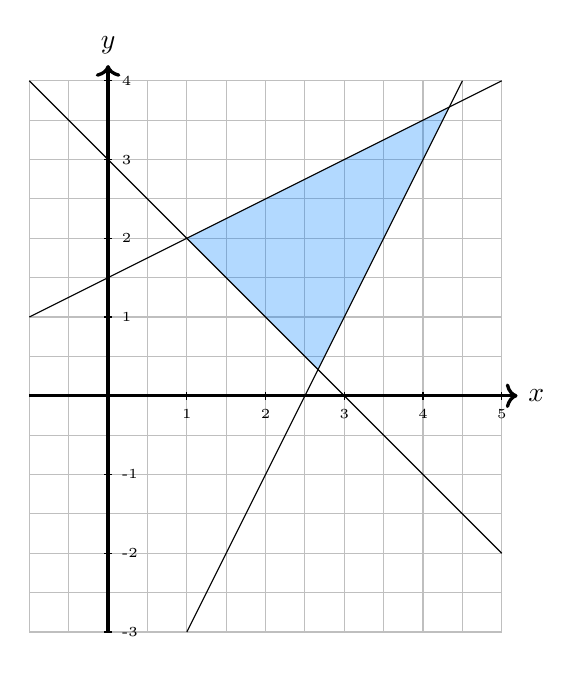
\begin{tikzpicture}

    \draw[gray!50, thin, step=0.5] (-1,-3) grid (5,4);
    \draw[very thick,->] (-1,0) -- (5.2,0) node[right] {$x$};
    \draw[very thick,->] (0,-3) -- (0,4.2) node[above] {$y$};

    \foreach \x in {1,...,5} \draw (\x,0.05) -- (\x,-0.05) node[below] {\tiny\x};
    \foreach \y in {1,...,4} \draw (-0.05,\y) -- (0.05,\y) node[right] {\tiny\y};
    \foreach \y in {-3,...,-1} \draw (-0.05,\y) -- (0.05,\y) node[right] {\tiny\y};

    \fill[blue!50!cyan,opacity=0.3] (8/3,1/3) -- (1,2) -- (13/3,11/3) -- cycle;

    \draw (-1,4) -- node[below,sloped] {} (5,-2);
    \draw (1,-3) -- (3,1) -- node[below left,sloped] {} (4.5,4);
    \draw (-1,1) -- node[above,sloped] {} (5,4);

\end{tikzpicture}

\begin{parts}
\part[1] Is this statement true or false?  One of the inequalities which define the feasible region is $\displaystyle y\leq -x+3$. 

\begin{oneparchoices}
\choice True \CorrectChoice False
\end{oneparchoices}
\part[1] Is this statement true or false?  One of the inequalities which define the feasible region is $\displaystyle y\geq 0.5x+3$. 

\begin{oneparchoices}
\choice True \CorrectChoice False
\end{oneparchoices}
\part[1] Is this statement true or false? If the objective function is $\displaystyle M=200-x-y$, then  the maximum of $M$ in the feasible region cannot be at $(3,2)$.

\begin{oneparchoices}
\CorrectChoice True \choice False
\end{oneparchoices}
\end{parts}

\question[1] Is this statement true or false? The system 

$\begin{cases} 3y-2x=0 \\ 4y+7x=0 \\  \end{cases}$
has exactly one solution.
\begin{oneparchoices}
\CorrectChoice True \choice False
\end{oneparchoices}

\question

Which of these functions are polynomial functions?

\begin{parts}
\part[1] $\displaystyle y=\frac{4+x^3}{x}$
\begin{oneparchoices}
\choice Polynomial \CorrectChoice Not polynomial
\end{oneparchoices}
\part[1] $\displaystyle y=\sqrt{x^2+2x+3}$
\begin{oneparchoices}
\choice Polynomial \CorrectChoice Not polynomial
\end{oneparchoices}
\part[1] $\displaystyle y=|x|$
\begin{oneparchoices}
\choice Polynomial \CorrectChoice Not polynomial
\end{oneparchoices}
\part[1] $\displaystyle y=x^2+\frac{2}{3}x+\sqrt{3}$
\begin{oneparchoices}
\CorrectChoice Polynomial \choice Not polynomial
\end{oneparchoices}
\end{parts}
\question[2] (Explanations are required.) The function $L(t)$ represents the number of landlines (per 100 people)  in a certain country $t$ years after 2010. What does the statement $L(3)=39$ mean in practical terms? [Do not write a formula for $L$.]
\begin{solution}
In 2013 there are 39 landlines per 100 people.
\end{solution}

\newpage

\question A community bird-watching society makes and sells simple bird feeders to raise money for its conservation activities. The material for each feeder cost \$6, and the society sells an average of 20 per week at a price of \$10 each. The society has been considering raising the price so it conducts a survey and finds that for every dollar increase, it loses 2 sales per week. The profit function is $\displaystyle P(x)=-2 x^2+52 x-240$, where $x$ is the price per feeder.

\begin{parts}
\part[2] (Explanations are required.) What price should the society charge for each feeder to maximize profit?
\begin{solution}
The profit $P$ is a quadratic function with negative leading coefficient, so the price that maximizes profit is the $x$ coordinate of the vertex, $\displaystyle \frac{-52}{-4}=13$. A table of values of $x$ and $P(x)$ is not sufficient, since the fact that $P(12)<P(13)$, $P(14)<P(13)$ is not sufficient to conclude that the required price is \$13. In fact, unless we use algebra, we cannot rule out the fact that the price could be \$13.2, or \$13.5 and so on.
\end{solution}
\part[2] (Explanations are required.) What is the maximum weekly profit?
\begin{solution}
Maximum profit: $P(13)=98$.
\end{solution}
\end{parts}
\question The quadratic function $f$ is given by the equation $\displaystyle f(x)=2x^2-4x-6$.

\begin{parts}
\part[3] (Explanations are required.) Find the coordinates of the vertex.
\begin{solution}
The vertex is $(1,-8)$. You can show your work in two different ways: (1) complete the square, write the standard form and find the vertex; or (2) find the $x$ coordinate of the vertex as $-b/(2a)$, and then substitute this number in the formula for $f$. It is not sufficient to graph (without showing (1) or (2)).
\end{solution}

\part[2] (Explanations are required.) Find the range of $f$ and write it in interval form.
\begin{solution}
Since the parabola opens up ($a=2>0$) the smallest number in the range is $-8$, which is the $y$ coordinate of the vertex. 
Range: $[-8,\infty)$
\end{solution}
\end{parts}

\question[4] Graph a function $f$ with domain $[-1,2]$ and range $[-2,1]$.
\begin{solution}
\begin{mfpic}[15]{-3}{3}{-3}{3}
    \polyline{(-1,-2),(2,1)};
    \point[3pt]{(-1,-2)}
    \point[3pt]{(2,1)}
\axes
\xmarks{-2,-1,1,2}
\ymarks{-2,-1,1,2}
\tlabel(3,-0.5){\scriptsize $x$}
\tlabel(0.5,3){\scriptsize $y$}
\axislabels {x}{{\tiny $-1 \hspace{7pt}$} -1, {\tiny $1$} 1, {\tiny $2$} 2}
\axislabels {y}{{\tiny $1$} 1, {\tiny $2$} 2}
\end{mfpic}

Any graph works, as long as: (1) the domain is $[-1,2]$ and the range is $[-2,1]$ and (2) the graph passes the vertical line test.
\end{solution}

\newpage

\question[3] (Explanations are required.) Graph the polynomial function $\displaystyle P(x)=-(x+1)^3+1$ using function transformations of $\displaystyle y=x^3$. Find the exact value of the $y$-intercept and show it on the graph. List all the transformations of $y=x^3$ (in the order that they are performed.)

\begin{solution}
The transformations are:
\begin{enumerate}
\item Reflection around the $x$ axis;
\item Horizontal shift by one unit to the left;
\item Vertical shift by one unit up.
\end{enumerate}
The $y$ coordinate of the $y$ intercept is $P(0)=0$.

\begin{mfpic}[15]{-3}{3}{-2}{5}
\arrow \reverse \arrow \function{-2.4,0.5, 0.1}{-((x+1)**3)+(1)} 
\axes
\tlabel[cc](3,-0.5){\scriptsize $x$}
\tlabel[cc](0.5,5){\scriptsize $y$}
\xmarks{-2,-1,1,2}
\ymarks{-2,-1,1,2}
\axislabels {x}{{\tiny $-1 \hspace{7pt}$} -1, {\tiny $1$} 1, {\tiny $2$} 2}
\axislabels {y}{{\tiny $1$} 1, {\tiny $2$} 2}
\end{mfpic}


\end{solution}

\bonusquestion[1] The domain of $\displaystyle f(x)=x^2+5x+6$ is: 
\begin{oneparchoices}
\choice $(-\infty,-3]\cup [-2,\infty)$
\choice $(-\infty,-3)\cup (-2,\infty)$
\choice $(-\infty,-3)\cup (-3,-2)\cup  (-2,\infty)$
\CorrectChoice $(-\infty,\infty)$
\choice None of these.
\end{oneparchoices}

\question[1] The domain of $\displaystyle f(x)=\frac{1}{x^2+5x+6}$ is:
 \begin{oneparchoices}
\choice $(-\infty,-3]\cup [-2,\infty)$
\choice $(-\infty,-3)\cup (-2,\infty)$
\CorrectChoice $(-\infty,-3)\cup (-3,-2)\cup  (-2,\infty)$
\choice $(-\infty,\infty)$
\choice None of these.
\end{oneparchoices}

\question[1] The domain of $\displaystyle f(x)=\sqrt{x^2+5x+6}$ is:
 \begin{oneparchoices}
\CorrectChoice $(-\infty,-3]\cup [-2,\infty)$
\choice $(-\infty,-3)\cup (-2,\infty)$
\choice $(-\infty,-3)\cup (-3,-2)\cup  (-2,\infty)$
\choice $(-\infty,\infty)$
\choice None of these.
\end{oneparchoices}

\question[1] The domain of $\displaystyle f(x)=\frac{1}{\sqrt{x^2+5x+6}}$ is:
 \begin{oneparchoices}
\choice $(-\infty,-3]\cup [-2,\infty)$
\CorrectChoice$(-\infty,-3)\cup (-2,\infty)$
\choice $(-\infty,-3)\cup (-3,-2)\cup  (-2,\infty)$
\choice $(-\infty,\infty)$
\choice None of these.
\end{oneparchoices}
\newpage

\question The goal of this problem is to graph the polynomial $\displaystyle P(x)=(x-1)^2(x+1)^3(x-2)$.
\begin{parts}
\part[1] What is the degree of $P$? 6
\part[1] What is the leading coefficient of $P$? 1
\part[1] How many $x$-intercept does the graph of $P$ have? 3
\part[1] What is the $y$-intercept? $(0,-2)$.
\part[5] (Explanations are required.) Graph $P$. 
\begin{solution}
The two tails of the graph point up because the degree is even and the leading coefficient is positive. The factor related to the $x$ intercept 1 appears with an even exponent, so the graph bounces off the $x$ axis at $x=-1$. The graph goes across the $x$ axis at the two other $x$ intercepts (-1 and 2) because the respective factors appear with odd exponents.

\begin{mfpic}[15]{-2}{3}{-5}{10}
\arrow \reverse \arrow \function{-1.4,2.2, 0.1}{((x-1)**2)*((x+1)**3)*((x-2)**1)} 
\axes
\tlabel[cc](3,-0.5){\scriptsize $x$}
\tlabel[cc](0.5,10){\scriptsize $y$}
\point[3pt]{(-1,0), (0,-2), (1,0), (2,0)}
\xmarks{-2,-1,1,2}
\ymarks{-2,-1,1,2}
\axislabels {x}{{\tiny $-1 \hspace{7pt}$} -1, {\tiny $1$} 1, {\tiny $2$} 2}
\axislabels {y}{{\tiny $1$} 1, {\tiny $2$} 2}
\end{mfpic}
\end{solution}

\end{parts}

\question[1] Write a formula for the function $f(x)$ obtained from $\displaystyle y=\sqrt{x}$ by applying the following transformations (in the given order): 
\begin{enumerate*}[series=MyList, before=\hspace{-0.6ex}] 
\item[(a)] reflection around the $y$ axis; \item[(b)] horizontal shift by 3 units to the left.
\end{enumerate*}

\begin{solution}
$f(x) =\sqrt{-(x+3)}$.  
\end{solution} 

\question[1] Write a formula for the function $g(x)$ obtained from $\displaystyle y=\sqrt{x}$ by applying the following transformations (in the given order): 
\begin{enumerate*}[series=MyList, before=\hspace{-0.6ex}] 
\item[(a)] horizontal shift by 3 units to the right;
\item[(b)] reflection around the $y$ axis.
\end{enumerate*}
\begin{solution}
$g(x) =\sqrt{-x-3}$  
\end{solution}
\bonusquestion[1] Assume that $f$ is a one-to-one function, and that $f(3)=11$. Then $\displaystyle f^{-1}(11)=3$

\end{questions}

\end{document}                 